%% ============================================================================
%% GECKO 2 — BMC Bioinformatics Manuscript (Springer Nature sn-jnl template)
%% Compile: pdflatex main && bibtex main && pdflatex main && pdflatex main
%% ============================================================================
\documentclass[pdflatex,sn-vancouver,Numbered]{sn-jnl}

%%%% Standard Packages
\usepackage{graphicx}
\usepackage{multirow}
\usepackage{amsmath,amssymb,amsfonts}
\usepackage{amsthm}
\usepackage{mathrsfs}
\usepackage[title]{appendix}
\usepackage{xcolor}
\usepackage{textcomp}
\usepackage{manyfoot}
\usepackage{booktabs}
\usepackage{algorithm}
\usepackage{algorithmicx}
\usepackage{algpseudocode}
\usepackage{listings}
\usepackage{tikz}
\usetikzlibrary{arrows.meta,positioning,shapes.geometric,fit,backgrounds}

\raggedbottom

%% Placeholder helper for pending Colab benchmark numbers (replaced automatically
%% by paper/populate_results.py once gecko2_paper_results.zip is provided).
\newcommand{\tbd}[1]{\textcolor{orange!75!black}{\texttt{[#1]}}}

%% ============================================================================
%% BENCHMARK RESULT MACROS (AUTO-UPDATED BY populate_results.py)
%% ============================================================================
% --- Hardware provenance ---
\newcommand{\hwCpu}{\tbd{CPU model / vCPUs}}
\newcommand{\hwRam}{\tbd{RAM}}
\newcommand{\hwGpu}{\tbd{NVIDIA Tesla T4 (16 GiB, sm\_75)}}
\newcommand{\hwRustc}{\tbd{rustc version}}
\newcommand{\hwGcc}{\tbd{gcc version}}
\newcommand{\hwNvcc}{\tbd{nvcc version}}

% --- Headline summary speedups (Abstract / Intro / Conclusions) ---
\newcommand{\hlChrOneSpeedupCpuVsVone}{\tbd{XX$\times$}}
\newcommand{\hlChrOneSpeedupCudaVsVone}{\tbd{XXX$\times$}}
\newcommand{\hlChrOneSpeedupCudaVsPub}{\tbd{XXXX$\times$}}
\newcommand{\hlChrOneVoneDiskGiB}{\tbd{XX.X~GiB}}
\newcommand{\hlAllVsAllCudaMin}{\tbd{X.X~min}}
\newcommand{\hlAllVsAllCudaSec}{\tbd{XXX.X~s}}
\newcommand{\hlAllVsAllSpeedupVsPubVone}{\tbd{XXX$\times$}}
\newcommand{\hlAllVsAllSpeedupVsMummer}{\tbd{XXXX$\times$}}
\newcommand{\hlWholeGenomeCudaSec}{\tbd{XX.X~s}}
\newcommand{\hlWholeGenomeCpuSec}{\tbd{XXX.X~s}}
\newcommand{\hlRustVsCfastPct}{\tbd{X.X\%}}
\newcommand{\hlExactParityPct}{\tbd{100.000\%}}
\newcommand{\hlVtwoRecoversVonePct}{\tbd{99.9+\%}}

% --- Experiment 1: Original 2015 Table 2 Replication (5 pairs x 5 backends) ---
% TYLCV (4 kb)
\newcommand{\eOneTylcvVone}{\tbd{t}}
\newcommand{\eOneTylcvCfast}{\tbd{t}}
\newcommand{\eOneTylcvCpu}{\tbd{t}}
\newcommand{\eOneTylcvWgpu}{\tbd{t}}
\newcommand{\eOneTylcvCuda}{\tbd{t}}
\newcommand{\eOneTylcvSp}{\tbd{s$\times$}}
\newcommand{\eOneTylcvDisk}{\tbd{d}}
\newcommand{\eOneTylcvFrags}{\tbd{n}}
% Buchnera (0.64 Mb)
\newcommand{\eOneBuchVone}{\tbd{t}}
\newcommand{\eOneBuchCfast}{\tbd{t}}
\newcommand{\eOneBuchCpu}{\tbd{t}}
\newcommand{\eOneBuchWgpu}{\tbd{t}}
\newcommand{\eOneBuchCuda}{\tbd{t}}
\newcommand{\eOneBuchSp}{\tbd{s$\times$}}
\newcommand{\eOneBuchDisk}{\tbd{d}}
\newcommand{\eOneBuchFrags}{\tbd{n}}
% E. coli (5 Mb)
\newcommand{\eOneEcoliVone}{\tbd{t}}
\newcommand{\eOneEcoliCfast}{\tbd{t}}
\newcommand{\eOneEcoliCpu}{\tbd{t}}
\newcommand{\eOneEcoliWgpu}{\tbd{t}}
\newcommand{\eOneEcoliCuda}{\tbd{t}}
\newcommand{\eOneEcoliSp}{\tbd{s$\times$}}
\newcommand{\eOneEcoliDisk}{\tbd{d}}
\newcommand{\eOneEcoliFrags}{\tbd{n}}
% Drosophila (20 Mb)
\newcommand{\eOneDrosVone}{\tbd{t}}
\newcommand{\eOneDrosCfast}{\tbd{t}}
\newcommand{\eOneDrosCpu}{\tbd{t}}
\newcommand{\eOneDrosWgpu}{\tbd{t}}
\newcommand{\eOneDrosCuda}{\tbd{t}}
\newcommand{\eOneDrosSp}{\tbd{s$\times$}}
\newcommand{\eOneDrosDisk}{\tbd{d}}
\newcommand{\eOneDrosFrags}{\tbd{n}}
% HS x PT chr1 (249 Mb x 228 Mb)
\newcommand{\eOneChrOneVone}{\tbd{t}}
\newcommand{\eOneChrOneCfast}{\tbd{t}}
\newcommand{\eOneChrOneCpu}{\tbd{t}}
\newcommand{\eOneChrOneWgpu}{\tbd{t}}
\newcommand{\eOneChrOneCuda}{\tbd{t}}
\newcommand{\eOneChrOneSp}{\tbd{s$\times$}}
\newcommand{\eOneChrOneDisk}{\tbd{d}}
\newcommand{\eOneChrOneTotWr}{\tbd{w}}
\newcommand{\eOneChrOneFrags}{\tbd{n}}
\newcommand{\eOneChrOneVoneFrags}{\tbd{n1}}
\newcommand{\eOneChrOneVtwoCovVone}{\tbd{p\%}}

% --- Experiment 2: Original 2015 Table 4 All-vs-All (45 pairs, 10 mammals) ---
\newcommand{\eTwoCudaWall}{\tbd{XXX.X}}
\newcommand{\eTwoCudaComp}{\tbd{XXX.X}}
\newcommand{\eTwoCudaRss}{\tbd{XXXX.X}}
\newcommand{\eTwoTotalFrags}{\tbd{N}}
\newcommand{\eTwoSpVoneCached}{\tbd{XXX$\times$}}
\newcommand{\eTwoSpVoneNocache}{\tbd{XXX$\times$}}
\newcommand{\eTwoSpMummer}{\tbd{XXXX$\times$}}
\newcommand{\eTwoSpGepard}{\tbd{XXXX$\times$}}
\newcommand{\eTwoSpLastz}{\tbd{XXXXX$\times$}}
% HS vs 9 mammals row (same-machine CPU vs CUDA)
\newcommand{\eTwoHsPtCpu}{\tbd{t}}  \newcommand{\eTwoHsPtCuda}{\tbd{t}}  \newcommand{\eTwoHsPtFrags}{\tbd{n}}
\newcommand{\eTwoHsMmCpu}{\tbd{t}}  \newcommand{\eTwoHsMmCuda}{\tbd{t}}  \newcommand{\eTwoHsMmFrags}{\tbd{n}}
\newcommand{\eTwoHsPaCpu}{\tbd{t}}  \newcommand{\eTwoHsPaCuda}{\tbd{t}}  \newcommand{\eTwoHsPaFrags}{\tbd{n}}
\newcommand{\eTwoHsGgCpu}{\tbd{t}}  \newcommand{\eTwoHsGgCuda}{\tbd{t}}  \newcommand{\eTwoHsGgFrags}{\tbd{n}}
\newcommand{\eTwoHsMmuCpu}{\tbd{t}} \newcommand{\eTwoHsMmuCuda}{\tbd{t}} \newcommand{\eTwoHsMmuFrags}{\tbd{n}}
\newcommand{\eTwoHsRnCpu}{\tbd{t}}  \newcommand{\eTwoHsRnCuda}{\tbd{t}}  \newcommand{\eTwoHsRnFrags}{\tbd{n}}
\newcommand{\eTwoHsBtCpu}{\tbd{t}}  \newcommand{\eTwoHsBtCuda}{\tbd{t}}  \newcommand{\eTwoHsBtFrags}{\tbd{n}}
\newcommand{\eTwoHsCfCpu}{\tbd{t}}  \newcommand{\eTwoHsCfCuda}{\tbd{t}}  \newcommand{\eTwoHsCfFrags}{\tbd{n}}
\newcommand{\eTwoHsSsCpu}{\tbd{t}}  \newcommand{\eTwoHsSsCuda}{\tbd{t}}  \newcommand{\eTwoHsSsFrags}{\tbd{n}}

% --- Experiment 3: Whole-Genome 24-Chr Human x Chimp (GRCh38.p14 x Clint_PTRv2) ---
\newcommand{\eThreeCfastWall}{\tbd{t}} \newcommand{\eThreeCfastComp}{\tbd{c}} \newcommand{\eThreeCfastRss}{\tbd{r}} \newcommand{\eThreeCfastRecall}{\tbd{p\%}}
\newcommand{\eThreeCpuWall}{\tbd{t}}   \newcommand{\eThreeCpuComp}{\tbd{c}}   \newcommand{\eThreeCpuRss}{\tbd{r}}   \newcommand{\eThreeCpuFrags}{\tbd{N}}
\newcommand{\eThreeWgpuWall}{\tbd{t}}  \newcommand{\eThreeWgpuComp}{\tbd{c}}  \newcommand{\eThreeWgpuRss}{\tbd{r}}  \newcommand{\eThreeWgpuRecall}{\tbd{p\%}}
\newcommand{\eThreeCudaWall}{\tbd{t}}  \newcommand{\eThreeCudaComp}{\tbd{c}}  \newcommand{\eThreeCudaRss}{\tbd{r}}  \newcommand{\eThreeCudaRecall}{\tbd{p\%}}
\newcommand{\eThreeCudaSpWall}{\tbd{s$\times$}}
\newcommand{\eThreeCudaSpComp}{\tbd{s$\times$}}
\newcommand{\eThreeWgpuSpWall}{\tbd{s$\times$}}
\newcommand{\eThreeCpuVsCfastSp}{\tbd{s$\times$}}

% --- Experiment 4A: Zero-Spill Slab Memory Scaling on HS chr1 x PT chr1 ---
\newcommand{\eFourACpuFiveTwelveW}{\tbd{t}} \newcommand{\eFourACpuFiveTwelveR}{\tbd{r}}
\newcommand{\eFourACpuOneGW}{\tbd{t}}       \newcommand{\eFourACpuOneGR}{\tbd{r}}
\newcommand{\eFourACpuTwoGW}{\tbd{t}}       \newcommand{\eFourACpuTwoGR}{\tbd{r}}
\newcommand{\eFourACpuFourGW}{\tbd{t}}      \newcommand{\eFourACpuFourGR}{\tbd{r}}
\newcommand{\eFourACudaFiveTwelveW}{\tbd{t}}\newcommand{\eFourACudaFiveTwelveR}{\tbd{r}}
\newcommand{\eFourACudaOneGW}{\tbd{t}}      \newcommand{\eFourACudaOneGR}{\tbd{r}}
\newcommand{\eFourACudaTwoGW}{\tbd{t}}      \newcommand{\eFourACudaTwoGR}{\tbd{r}}
\newcommand{\eFourACudaFourGW}{\tbd{t}}     \newcommand{\eFourACudaFourGR}{\tbd{r}}

% --- Experiment 4B: (WL, FL) Sensitivity Frontier on Drosophila 2R x 3 ---
\newcommand{\eFourBWTwelveFTwentyCpu}{\tbd{t}}    \newcommand{\eFourBWTwelveFTwentyCuda}{\tbd{t}}    \newcommand{\eFourBWTwelveFTwentySp}{\tbd{s$\times$}}    \newcommand{\eFourBWTwelveFTwentyFrags}{\tbd{n}}
\newcommand{\eFourBWTwelveFThouCpu}{\tbd{t}}      \newcommand{\eFourBWTwelveFThouCuda}{\tbd{t}}      \newcommand{\eFourBWTwelveFThouSp}{\tbd{s$\times$}}      \newcommand{\eFourBWTwelveFThouFrags}{\tbd{n}}
\newcommand{\eFourBWSixteenFTwentyCpu}{\tbd{t}}   \newcommand{\eFourBWSixteenFTwentyCuda}{\tbd{t}}   \newcommand{\eFourBWSixteenFTwentySp}{\tbd{s$\times$}}   \newcommand{\eFourBWSixteenFTwentyFrags}{\tbd{n}}
\newcommand{\eFourBWSixteenFThouCpu}{\tbd{t}}     \newcommand{\eFourBWSixteenFThouCuda}{\tbd{t}}     \newcommand{\eFourBWSixteenFThouSp}{\tbd{s$\times$}}     \newcommand{\eFourBWSixteenFThouFrags}{\tbd{n}}
\newcommand{\eFourBWTwentyFourFTwentyCpu}{\tbd{t}}\newcommand{\eFourBWTwentyFourFTwentyCuda}{\tbd{t}}\newcommand{\eFourBWTwentyFourFTwentySp}{\tbd{s$\times$}}\newcommand{\eFourBWTwentyFourFTwentyFrags}{\tbd{n}}
\newcommand{\eFourBWThirtyTwoFTwentyCpu}{\tbd{t}} \newcommand{\eFourBWThirtyTwoFTwentyCuda}{\tbd{t}} \newcommand{\eFourBWThirtyTwoFTwentySp}{\tbd{s$\times$}} \newcommand{\eFourBWThirtyTwoFTwentyFrags}{\tbd{n}}
%% ============================================================================

\begin{document}

\title[GECKO 2: Zero-Disk, GPU-Accelerated Whole-Genome Pairwise Comparison]{GECKO 2: Breaking the Memory, Disk, and Accelerator Barriers of Whole-Genome Pairwise Comparison}

\author*[1]{\fnm{Oscar} \sur{Torreno}}\email{otorreno@uma.es}
\author[1]{\fnm{Oswaldo} \sur{Trelles}}\email{ots@ac.uma.es}

\affil*[1]{\orgdiv{Computer Architecture Department}, \orgname{University of M\'alaga}, \orgaddress{\street{Bulevar Louis Pasteur 35}, \city{M\'alaga}, \postcode{29071}, \country{Spain}}}

%% ============================================================================
%% STRUCTURED ABSTRACT (BMC Bioinformatics format: Background / Results / Conclusions)
%% ============================================================================
\abstract{%
\textbf{Background:} Exhaustive pairwise whole-genome comparison for High-scoring Segment Pair (HSP) detection remains a cornerstone of comparative genomics, synteny analysis, and structural rearrangement discovery. The original GECKO software overcame the main-memory limits of suffix-array aligners through a modular out-of-core disk pipeline, enabling mammalian chromosome comparisons on commodity hardware. However, writing and externally sorting tens to hundreds of gigabytes of intermediate $k$-mer dictionaries and seed hit lists has become the dominant performance and storage bottleneck on modern multi-core CPUs, cloud instances, and GPUs.

\textbf{Results:} We present GECKO~2, a ground-up Rust and GPU-accelerated re-architecture that replaces GECKO's external dual-dictionary merge-sort pipeline with a zero-disk, memory-bounded, single-reference streaming engine. Sequences are stored in a 2-bit packed representation ($0.25\text{ bytes/bp}$ on host, $0.375\text{ bytes/bp}$ on GPU) paired with sparse run-length annotations for ambiguous bases and multi-FASTA boundaries. Only the reference genome is indexed once using canonical $k$-mers via Direct-CSR or 2-level parallel radix-partitioned Hash-CSR tables, automatically sliced into zero-spill memory-bounded slabs under a user-specified RAM budget. On CPUs, GECKO~2 combines lock-free streaming lookup, a 2-tier Fibonacci-hashed diagonal cache, mathematically exact rejected-span skipping, and 2-bit SWAR/AVX2 bidirectional extension, outperforming an optimized \texttt{-march=native} C in-memory baseline by \hlRustVsCfastPct{} while maintaining \hlExactParityPct{} bit-exact fragment parity. On GPUs, native CUDA (using on-device CUB radix sort, lock-free left/right-maximal seed filtering, and two-tier warp-cooperative 2-bit extension) and cross-vendor WebGPU (\texttt{wgpu}) backends accelerate mammalian comparisons further. Replicating the exact five pairwise datasets from Torreno \& Trelles (2015) across 4~kb to 249~Mb, GECKO~2 achieves up to \hlChrOneSpeedupCpuVsVone{} CPU and \hlChrOneSpeedupCudaVsVone{} CUDA speedups over Legacy GECKO~v1 on identical hardware while reducing temporary disk I/O from \hlChrOneVoneDiskGiB{} to 0~B. On the original 45-pair, 10-species mammalian chromosome~1 all-versus-all benchmark (39.7~h on GECKO~v1 and 6.5--55~days on MUMmer/Gepard/LASTZ in 2015), GECKO~2 CUDA completes all 45 comparisons in \hlAllVsAllCudaMin{} on a single T4 GPU. Furthermore, an entire 24-chromosome \textit{Homo sapiens} versus \textit{Pan troglodytes} genome comparison ($\sim$3.1~Gb $\times$ 2.9~Gb) finishes in \hlWholeGenomeCudaSec{} on CUDA and \hlWholeGenomeCpuSec{} on CPU.

\textbf{Conclusions:} GECKO~2 eliminates external disk I/O, bounds memory strictly even on 250~Mb chromosomes inside 512~MiB RAM, and brings interactive whole-genome HSP detection to commodity CPUs and GPUs while preserving drop-in compatibility with legacy binary \texttt{.frags} and GECKO-MGV workflows.}

\keywords{Comparative genomics, Pairwise genome comparison, High-scoring Segment Pairs, GPU acceleration, CUDA, WebGPU, Rust, Memory-bounded streaming}

\maketitle

%% ============================================================================
%% 1. BACKGROUND
%% ============================================================================
\section{Background}\label{sec:background}

Pairwise whole-genome comparison is a foundational operation in comparative genomics, underpinning the discovery of conserved synteny blocks, chromosomal rearrangements (inversions, translocations, duplications), repeat families, and evolutionary distances across all domains of life. Classical dynamic programming algorithms for global \cite{needleman1970} and local \cite{smith1981} sequence alignment scale quadratically in time and space, rendering them infeasible for megabase- and gigabase-scale genomes. Modern whole-genome comparison methods therefore rely on seed-and-extend heuristics pioneered by FASTA \cite{pearson1988fasta} and BLAST \cite{altschul1990blast}, implemented via suffix trees/arrays, hash indices, or minimizer sketches in tools such as MegaBLAST \cite{zhang2000megablast}, MUMmer \cite{kurtz2004mummer,marcais2018mummer4}, Gepard \cite{krumsiek2007gepard}, Mauve \cite{darling2004mauve}, LASTZ \cite{harris2007lastz}, LAST \cite{kielbasa2011last}, and minimap2 \cite{li2018minimap2}.

In 2015, we introduced GECKO (GEnome Comparison with $K$-mers Out-of-core) \cite{torreno2015gecko} to address the severe main-memory limits faced by suffix-array-based aligners on mammalian chromosomes. Unlike tools that required 15--300~GB of RAM to compare 250~Mb chromosomes, GECKO~v1 adopted a modular out-of-core strategy that partitioned $k$-mer dictionaries, sorted seed matches (hits), and streamed ungapped High-scoring Segment Pair (HSP) extensions through secondary storage. While GECKO~v1 successfully enabled chromosome-scale comparisons within $\sim$1.6~GB of RAM and became integrated into downstream visual analytics platforms such as GECKO-MGV \cite{diazdelpino2019geckomgv} and coarse-grained companions such as CHROMEISTER \cite{perezwohlfeil2019chromeister}, its disk-centric design carries heavy costs on contemporary hardware:
\begin{enumerate}
    \item \textbf{Severe intermediate disk amplification:} GECKO~v1 constructs three full on-disk 32-mer dictionaries (query $X$, reference $Y$, and reverse-complement $\bar{Y}$), materializes raw hit lists, externally merges and sorts them, and filters them before extension. A single mammalian chromosome pair writes tens to hundreds of gigabytes of temporary files (up to $\sim$600~GB for closely related human--gorilla chromosomes under default settings), saturating shared cluster filesystems and cloud ephemeral volumes.
    \item \textbf{High fixed overhead on small genomes:} Building disk dictionaries and allocating fixed memory pools caused GECKO~v1 to lag in-memory suffix-array aligners on viral and bacterial genomes (4~kb--5~Mb).
    \item \textbf{Underutilization of modern multi-core CPUs and GPUs:} Apart from multi-threaded external quicksort, GECKO~v1's dictionary extraction, hit matching, filtering, and HSP extension stages were largely sequential and I/O-bound, unable to exploit SIMD vector units or massively parallel GPU accelerators.
    \item \textbf{Memory-safety and maintenance debt:} Legacy C code harbored subtle defects such as an 8~MiB stack-allocated offset array in \texttt{reverseComplement.c}, an off-by-one matrix index overflow at 100\% similarity, and a shell-wrapper hardcoded frequency limit (\texttt{FL=1000}).
\end{enumerate}

At the same time, genome sequencing throughput has continued to outpace single-thread CPU scaling, while commodity workstations and cloud notebooks routinely provide multi-core AVX2/NEON CPUs and discrete GPUs (NVIDIA CUDA as well as cross-vendor Vulkan/Metal/DirectX~12 hardware). Re-thinking GECKO for this hardware landscape requires moving beyond retrofitting disk I/O and instead redesigning the data representation, indexing model, diagonal deduplication, and extension kernels from first principles.

In this article, we present \textbf{GECKO~2}, a memory-safe Rust and GPU-accelerated re-architecture of GECKO that eliminates temporary disk I/O completely while preserving exact ungapped HSP semantics and drop-in binary \texttt{.frags} compatibility. Our principal contributions are:
\begin{itemize}
    \item \textbf{Single-reference canonical indexing with zero-spill memory-bounded slabs:} Indexing only reference $Y$ once with canonical $k$-mers and automatically partitioning large references into RAM-budgeted slabs (\texttt{-m 512M} to \texttt{4G+}) guarantees 0~B temporary disk usage and deterministic memory ceilings even on 250~Mb mammalian chromosomes.
    \item \textbf{2-bit packed DNA with sparse run-length annotations (host and GPU):} Storing sequences at $0.25\text{ bytes/bp}$ on host ($0.375\text{ bytes/bp}$ on GPU including 1-bit special/invalid masks) reduces memory bandwidth by up to $4\times$ and enables 32-bp word-parallel exact-match fast paths during ungapped extension.
    \item \textbf{Algorithmic CPU acceleration in portable Rust:} Combining a 2-level parallel radix-partitioned Hash-CSR index, non-polluting L2/L3 software prefetching, a 2-tier Fibonacci-hashed diagonal cache, exact rejected-span skipping, and 2-bit SWAR/AVX2 extension allows portable Rust to surpass a hand-tuned \texttt{-O3 -march=native} C in-memory baseline by \hlRustVsCfastPct{} at \hlExactParityPct{} bit-exact fragment parity.
    \item \textbf{Dual GPU backends (native CUDA and cross-vendor WebGPU):} Native CUDA performs on-device 2-bit reverse-complementation, CUB radix sorting, lock-free left/right-maximal seed filtering, and two-tier warp-cooperative 2-bit extension; a companion \texttt{wgpu} WGSL backend provides vendor-agnostic GPU acceleration across Vulkan, Metal, and DirectX~12.
\end{itemize}

To establish direct continuity with the original publication, we evaluate GECKO~2 on the \textbf{exact five pairwise datasets} (4~kb--249~Mb) and the \textbf{exact 10-species, 45-pair mammalian chromosome~1 all-versus-all dataset} from Torreno \& Trelles (2015) \cite{torreno2015gecko}, and further demonstrate whole-genome 24-chromosome human-versus-chimpanzee comparison, strict slab-memory scaling down to 512~MiB, and dense short-seed sensitivity ablations.

%% ============================================================================
%% 2. IMPLEMENTATION
%% ============================================================================
\section{Implementation}\label{sec:implementation}

GECKO~2 is implemented as a modular Rust workspace \cite{matsakis2014rust} comprising four crates: \texttt{gecko-core} (sequence representation, canonical indexing, streaming CPU engine, and legacy/modern I/O formats), \texttt{gecko-cuda} (native NVIDIA CUDA + CUB kernels linked via C FFI), \texttt{gecko-wgpu} (portable WebGPU/WGSL compute pipelines), and \texttt{gecko-cli} (unified command-line interface with automatic backend dispatch and end-to-end parity tests).

\subsection{From external dual-dictionary merge-sort to single-reference streaming}\label{subsec:arch}

Figure~\ref{fig:architecture} contrasts Legacy GECKO~v1 with GECKO~2. GECKO~v1 required eight distinct executable stages communicating exclusively through intermediate disk files: reverse-complementing $Y$, extracting unsorted 32-mer streams for $X$, $Y$, and $\bar{Y}$, externally sorting all three streams, converting each sorted stream into paired hash-dictionary files (\texttt{.d2hW}/\texttt{.d2hP}), joining dictionaries to emit raw hit files for both strands, externally sorting hits by diagonal, filtering proximal hits, and finally extending surviving seeds via random disk-backed sequence reads.

GECKO~2 collapses this entire workflow into a single zero-disk streaming pass:
\begin{enumerate}
    \item Both FASTA (or gzip-compressed \texttt{.fa.gz}) inputs are parsed once into compact 2-bit \texttt{PackedSeq} buffers in RAM.
    \item Only reference $Y$ is indexed at the requested seed length $k \in [4, 32]$ (removing v1's multiple-of-4 restriction) using canonical $k$-mers, automatically partitioned into disjoint coordinate slabs whenever the full index would exceed the user's memory budget \texttt{-m}.
    \item Query $X$ is streamed in parallel chunks directly against each reference slab, computing forward and reverse-complement matches simultaneously, deduplicating diagonals on the fly, and performing exact bidirectional ungapped HSP extension against the full 2-bit sequences.
\end{enumerate}

\begin{figure}[t]
\centering
\resizebox{\textwidth}{!}{%
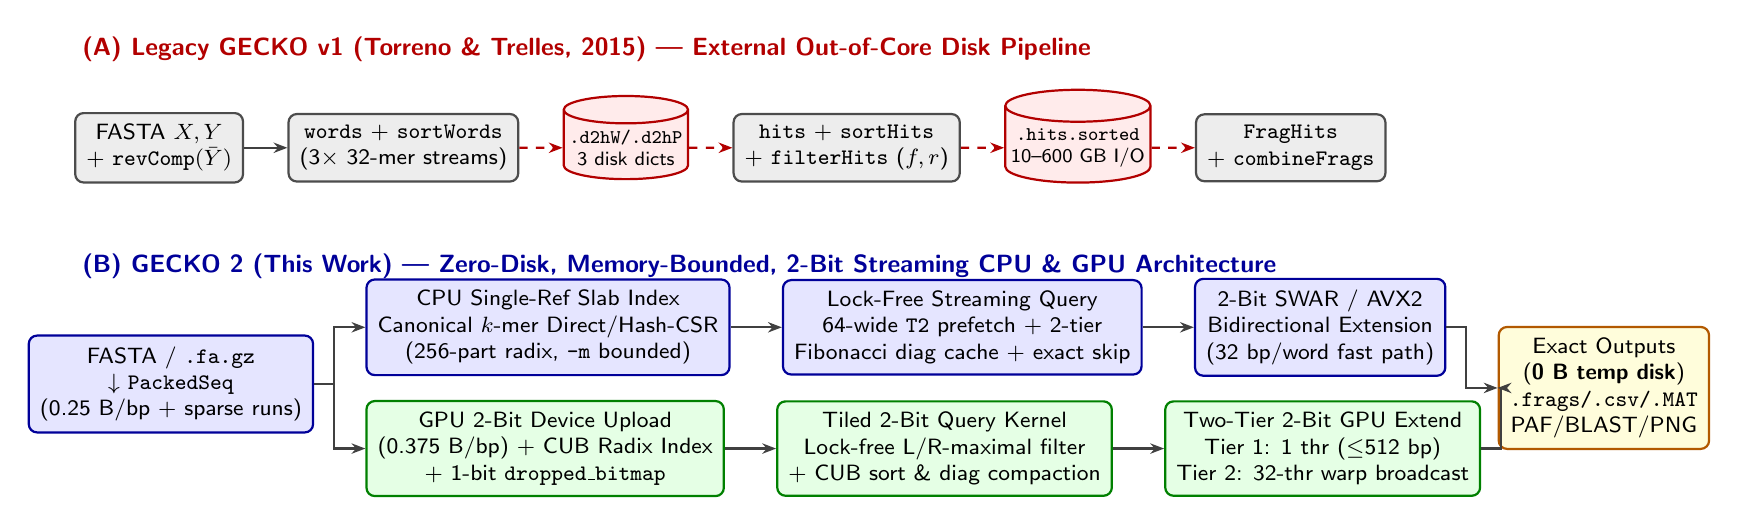
\begin{tikzpicture}[
    node distance=0.45cm and 0.55cm,
    box/.style={rectangle, rounded corners=3pt, draw=black!70, thick, minimum height=0.82cm, align=center, font=\sffamily\footnotesize, inner sep=4pt},
    disk/.style={cylinder, shape border rotate=90, aspect=0.22, draw=red!70!black, fill=red!8, thick, minimum height=0.78cm, minimum width=1.45cm, align=center, font=\sffamily\scriptsize, inner sep=2pt},
    v1/.style={box, fill=gray!14, minimum width=1.95cm},
    v2cpu/.style={box, fill=blue!10, draw=blue!60!black, minimum width=2.25cm},
    v2gpu/.style={box, fill=green!10, draw=green!50!black, minimum width=2.25cm},
    arr/.style={-{Stealth[length=5pt]}, thick, draw=black!75},
    darr/.style={-{Stealth[length=5pt]}, thick, dashed, draw=red!70!black},
]
% --- Row 1: Legacy GECKO v1 ---
\node[font=\sffamily\bfseries\small, anchor=west, text=red!70!black] (lbl1) at (0, 2.60) {(A) Legacy GECKO v1 (Torreno \& Trelles, 2015) --- External Out-of-Core Disk Pipeline};

\node[v1] (v1in) at (1.1, 1.35) {FASTA $X, Y$\\+ \texttt{revComp}$(\bar{Y})$};
\node[v1, right=of v1in] (v1w) {\texttt{words} + \texttt{sortWords}\\(3$\times$ 32-mer streams)};
\node[disk, right=of v1w] (v1d1) {\texttt{.d2hW/.d2hP}\\3 disk dicts};
\node[v1, right=of v1d1] (v1h) {\texttt{hits} + \texttt{sortHits}\\+ \texttt{filterHits} ($f,r$)};
\node[disk, right=of v1h] (v1d2) {\texttt{.hits.sorted}\\10--600 GB I/O};
\node[v1, right=of v1d2] (v1f) {\texttt{FragHits}\\+ \texttt{combineFrags}};

\draw[arr] (v1in) -- (v1w);
\draw[darr] (v1w) -- (v1d1);
\draw[darr] (v1d1) -- (v1h);
\draw[darr] (v1h) -- (v1d2);
\draw[darr] (v1d2) -- (v1f);

% --- Row 2: GECKO 2 ---
\node[font=\sffamily\bfseries\small, anchor=west, text=blue!60!black] (lbl2) at (0, -0.15) {(B) GECKO 2 (This Work) --- Zero-Disk, Memory-Bounded, 2-Bit Streaming CPU \& GPU Architecture};

\node[v2cpu] (v2in) at (1.25, -1.65) {FASTA / \texttt{.fa.gz}\\$\downarrow$ \texttt{PackedSeq}\\(0.25~B/bp + sparse runs)};
\node[v2cpu, right=0.65cm of v2in, yshift=0.72cm] (v2idx) {CPU Single-Ref Slab Index\\Canonical $k$-mer Direct/Hash-CSR\\(256-part radix, \texttt{-m} bounded)};
\node[v2cpu, right=0.65cm of v2idx] (v2str) {Lock-Free Streaming Query\\64-wide \texttt{T2} prefetch + 2-tier\\Fibonacci diag cache + exact skip};
\node[v2cpu, right=0.65cm of v2str] (v2ext) {2-Bit SWAR / AVX2\\Bidirectional Extension\\(32~bp/word fast path)};

\node[v2gpu, right=0.65cm of v2in, yshift=-0.82cm] (gidx) {GPU 2-Bit Device Upload\\(0.375~B/bp) + CUB Radix Index\\+ 1-bit \texttt{dropped\_bitmap}};
\node[v2gpu, right=0.65cm of gidx] (gqry) {Tiled 2-Bit Query Kernel\\Lock-free L/R-maximal filter\\+ CUB sort \& diag compaction};
\node[v2gpu, right=0.65cm of gqry] (gext) {Two-Tier 2-Bit GPU Extend\\Tier~1: 1 thr ($\le$512~bp)\\Tier~2: 32-thr warp broadcast};

\node[box, fill=yellow!14, draw=orange!70!black, right=0.65cm of v2ext, yshift=-0.77cm, minimum width=2.05cm] (out) {Exact Outputs\\(\textbf{0~B temp disk})\\\texttt{.frags/.csv/.MAT}\\PAF/BLAST/PNG};

\draw[arr] (v2in.east) -- ++(0.25,0) |- (v2idx.west);
\draw[arr] (v2in.east) -- ++(0.25,0) |- (gidx.west);
\draw[arr] (v2idx) -- (v2str);
\draw[arr] (v2str) -- (v2ext);
\draw[arr] (gidx) -- (gqry);
\draw[arr] (gqry) -- (gext);
\draw[arr] (v2ext.east) -- ++(0.25,0) |- (out.west);
\draw[arr] (gext.east) -- ++(0.25,0) |- (out.west);
\end{tikzpicture}%
}
\caption{Architectural comparison between Legacy GECKO~v1 and GECKO~2. \textbf{(A)} Legacy GECKO~v1 relies on three full on-disk 32-mer dictionaries and externally sorted hit files, writing tens to hundreds of gigabytes of temporary I/O on mammalian chromosomes. \textbf{(B)} GECKO~2 encodes both sequences once in a 2-bit packed representation, indexes only reference $Y$ in memory-bounded canonical slabs, and executes either a lock-free streaming CPU pipeline or native CUDA / cross-vendor WebGPU compute pipelines with zero temporary disk I/O while producing bit-exact legacy \texttt{.frags} and modern alignment formats.}\label{fig:architecture}
\end{figure}

\subsection{2-Bit packed DNA with sparse run-length annotations}\label{subsec:packedseq}

Storing DNA as 1-byte ASCII arrays consumes $\sim$500~MB just to hold two 250~Mb mammalian chromosomes and forces byte-by-byte comparisons during HSP extension. In GECKO~2, \texttt{PackedSeq} stores bases at $0.25\text{ bytes/bp}$ (32 bases per little-endian \texttt{u64} word, encoding $\text{A}=00_2$, $\text{C}=01_2$, $\text{G}=10_2$, $\text{T/U}=11_2$ so bitwise complementation maps $\text{A}\leftrightarrow\text{T}$ and $\text{C}\leftrightarrow\text{G}$ via \texttt{x \^{} 3}). Two trailing sentinel \texttt{0u64} words allow any unaligned 32-base window $[p, p+32)$ to be loaded branchlessly in a single shifted 128-bit funnel shift (\texttt{load\_32}), while reverse windows $[p-31, p]$ are obtained by a 3-instruction SWAR 2-bit lane reversal (\texttt{reverse\_32\_2bit}).

To preserve 100\% exact legacy handling of ambiguous bases, soft-masking, and multi-FASTA boundaries without inflating the dense base array, non-canonical symbols are recorded in compact sorted run-length vectors: \texttt{n\_runs} (half-open intervals of `\texttt{N}'/`\texttt{n}'), \texttt{soft\_runs} (soft-masked lowercase runs), \texttt{sep\_pos} (multi-FASTA record separators \texttt{SEQ\_SEP}), and \texttt{iupac} (rare non-ACGTN IUPAC bytes). Their coalesced union \texttt{special\_runs} lets the extension loop query the exact distance to the next special character in $O(\log |\text{special\_runs}|)$ once per span, remaining inside a pure 2-bit register loop across long clean stretches.

On GPU devices, each \texttt{PackedSeq} is mirrored as a \texttt{GpuSeqView} consisting of the 2-bit \texttt{uint64\_t} word array ($0.25\text{ bytes/bp}$) plus two compact 1-bit-per-base bitmaps ($0.0625\text{ bytes/bp}$ each): \texttt{invalid\_bm} (for $k$-mer seed exclusion) and \texttt{special\_bm} (for extension slow-path dispatch), yielding a total GPU sequence footprint of only $0.375\text{ bytes/bp}$ (2.67$\times$ smaller than ASCII) while accelerating extension memory bandwidth by up to $4\times$.

\subsection{Single-reference canonical indexing and zero-spill memory-bounded slabs}\label{subsec:refindex}

Rather than building separate forward and reverse-complement dictionaries for both $X$ and $Y$, GECKO~2 indexes only reference $Y$ once. At each valid position $p_y$ of $Y$, rolling forward ($k_f$) and reverse-complement ($k_r$) 2-bit $k$-mers are maintained in $O(1)$ per base, and the canonical key $c = \min(k_f, k_r)$ is stored together with a packed occurrence entry $(p_y \ll 1) \mid s_y$, where $s_y = \mathbb{I}[k_r < k_f]$ records the canonical orientation (\texttt{u32} for $|Y| < 2^{31}$~bp, with automatic \texttt{u64} fallback for $>2.1$~Gb concatenated references). Two CSR index layouts are selected automatically:
\begin{itemize}
    \item \textbf{Direct-CSR (small $k$):} When $4^k$ buckets fit cheaply within the budget, \texttt{offsets} is indexed directly by $c$ with zero key storage, reducing each lookup to two array reads.
    \item \textbf{2-Level Parallel Radix-Partitioned Hash-CSR (large $k \le 32$):} Each canonical key is mixed with the invertible 64-bit MurmurHash3 finalizer $h = \text{fmix64}(c)$ \cite{appleby2011murmurhash3}. Reference positions are partitioned across 256 top-level radix buckets in parallel via Rayon, counted, scattered into cache-resident sub-buckets, sorted locally by $h$, and filtered per strand against \texttt{freq\_limit} (discarding words whose frequency on a given strand exceeds \texttt{FL}). Per-partition sentinel slots eliminate boundary branches during range lookups.
\end{itemize}

\paragraph{Zero-spill reference-slab partitioning.}
When a reference chromosome would cause the Hash-CSR tables and scatter buffers to exceed the user's memory budget $M$ (flag \texttt{-m}, default \texttt{2G}, tested down to \texttt{512M}), GECKO~2 automatically computes the maximum safe slab length $L_{\text{slab}}(M)$ from the exact per-base byte cost of the CSR arrays and partitions $Y$ into $\lceil |Y| / L_{\text{slab}} \rceil$ disjoint slabs. Each slab is indexed and queried in turn while keeping both compact 2-bit \texttt{PackedSeq} sequences resident, ensuring that HSP extensions crossing slab boundaries extend seamlessly over the full sequences and produce bit-identical results regardless of $M$ with \textbf{zero disk spillover}.

\paragraph{Single-reference vs.\ dual-dictionary frequency filtering.}
A subtle algorithmic distinction exists between Legacy GECKO~v1 and single-reference streaming engines (both \texttt{c\_fast} and GECKO~2). Legacy GECKO~v1's \texttt{hits} module skips any $k$-mer whose multiplicity exceeds \texttt{FL} in \emph{either} $X$ or $Y$, whereas single-reference indexing skips $k$-mers whose per-strand multiplicity exceeds \texttt{FL} in reference $Y$ only. Consequently, GECKO~2 retains valid HSPs where a duplicated region in query $X$ matches a unique locus in reference $Y$ (typically $+1\%$ additional fragments on primate chromosomes) while recovering virtually $100\%$ of Legacy GECKO~v1's fragments. We report bidirectional parity metrics explicitly in Section~\ref{sec:results}.

\subsection{Lock-free streaming CPU engine}\label{subsec:cpu}

Query $X$ is partitioned dynamically into $\sim$1~Mb Rayon chunks processed concurrently with zero cross-thread locks:
\begin{enumerate}
    \item \textbf{64-wide batched lookup with non-polluting prefetching:} Rolling canonical query $k$-mers are buffered in batches of 64. Before probing, each bucket offset is prefetched with \texttt{\_mm\_prefetch(\_MM\_HINT\_T2)} into L2/L3 cache rather than L1d, preventing random CSR probes from evicting the hot diagonal cache.
    \item \textbf{2-tier Fibonacci-hashed diagonal cache (\texttt{StrandDiagCache}):} Each worker thread maintains two direct-mapped tables per strand indexed by $(d \cdot \phi_{64}) \gg (64 - b)$ (where $d = p_x - p_y$ on the forward strand, $\phi_{64} = \text{0x9E3779B97F4A7C15}$): a 2~MiB \texttt{hsp} tier ($2^{17}$ slots) tracking the furthest covered $x$-coordinate of accepted HSPs and exact reject bounds, and a separate 1~MiB \texttt{noise} tier ($2^{16}$ slots) for short failed seeds so transient repeat noise cannot evict active long HSP diagonals.
    \item \textbf{Mathematically exact rejected-span skipping:} Whenever a seed at $(p_x, p_y)$ extends forward and backward to a local maximum that fails the length ($L$) or similarity ($S$) threshold, naive streaming would re-extend every subsequent collinear seed along the same diagonal. GECKO~2 computes a linear-time block min/max and suffix-minimum envelope over the rejected extension's score profile to determine the exact rightmost coordinate $x_{\text{skip}}$ such that no seed in $[p_x, x_{\text{skip}}]$ on diagonal $d$ can exceed the failing HSP's score, recording $x_{\text{skip}}$ in the diagonal cache without losing a single valid fragment.
    \item \textbf{2-bit SWAR / AVX2+BMI2 bidirectional ungapped extension:} Matching GECKO's exact scoring model ($+4$ match, $-4$ mismatch, $-1$ for `\texttt{N}', immediate stop at \texttt{SEQ\_SEP}), extension operates on 32-base 2-bit words (\texttt{wx}, \texttt{wy}). On special-free spans, identical 32-base words (\texttt{wx == wy}) advance by 32~bp in a single branchless step ($+128$ score, $+32$ identities); otherwise 2-bit XOR + popcount/AVX2+BMI2 extracts match masks across 32 bases at a time, automatically compiling cleanly on portable x86\_64/ARM64 targets with runtime feature dispatch.
\end{enumerate}

\subsection{Native NVIDIA CUDA backend (\texttt{gecko-cuda})}\label{subsec:cuda}

The native CUDA backend executes the complete indexing, seeding, filtering, and ungapped extension pipeline on the GPU in three stages:
\begin{itemize}
    \item \textbf{Stage 1 --- On-device 2-bit indexing (\texttt{cuda\_index.cu}):} After uploading 2-bit \texttt{PackedSeq} buffers ($0.375\text{ bytes/bp}$), a word-level kernel generates $\bar{Y}$ directly in 2-bit form via \texttt{\~{}reverse\_32\_2bit} and bit-reverses the 1-bit \texttt{special\_bm} via \texttt{\_\_brev}. Canonical $k$-mers are extracted in parallel, sorted with CUB \texttt{DeviceRadixSort::SortPairs} \cite{merrill2015cub}, compacted with exact per-strand \texttt{freq\_limit} filtering, and accompanied by a 1-bit \texttt{dropped\_bitmap} marking reference positions whose $k$-mer exceeded \texttt{FL}.
    \item \textbf{Stage 2 --- Tiled 2-bit query \& lock-free left/right-maximal seed filtering (\texttt{cuda\_query.cu}):} Query $X$ is swept in tiles where each thread processes a 16-bp stride, probes the bucketed \texttt{fmix64} CSR via read-only texture cache (\texttt{\_\_ldg}), and immediately tests whether each hit $(p_x, p_y)$ extends by 1~bp to the left \emph{and} right in 2-bit \texttt{seqX}/\texttt{seqY} (checking \texttt{dropped\_bitmap} so filtered neighbors do not suppress valid boundary seeds). Interior hits of long exact runs are discarded in registers with zero global-memory atomics, cutting raw hit volume by an order of magnitude. Surviving boundary seeds are packed into 64-bit diagonal-ordered keys, sorted via CUB \texttt{RadixSort}, and proximity-compacted per diagonal.
    \item \textbf{Stage 3 --- Two-tier 2-bit GPU bidirectional extension (\texttt{cuda\_extend.cu}):} Because HSP lengths follow a heavy-tailed distribution (millions of short noisy seeds vs.\ thousands of multi-kilobase syntenic blocks), a uniform 1-thread-per-seed kernel suffers severe warp divergence. GECKO~2 therefore splits extension into two tiers:
    \begin{itemize}
        \item \emph{Tier~1 (Short, 1 thread/seed, 512~bp cap):} Extends using 32-base word-loaded register stepping with a 1-step 32-bp exact-match fast path. Over 95\% of seeds terminate or resolve within 512~bp; any seed reaching the cap is pushed to a compact \texttt{long\_seeds} queue.
        \item \emph{Tier~2 (Long, 32-thread warp/seed):} Assigns a full 32-thread warp per long seed, loading a single warp-broadcast 64-bit word per 32~bp, exploiting a 1-cycle 32-bp exact-match fast path, and computing exact peak scores and endpoints via zero-divergence warp prefix sums (\texttt{\_\_shfl\_up\_sync}).
    \end{itemize}
    Only fragments passing $(L, S)$ are copied back to host memory for final diagonal deduplication and output serialization.
\end{itemize}

\subsection{Cross-vendor WebGPU backend (\texttt{gecko-wgpu})}\label{subsec:wgpu}

To avoid proprietary CUDA lock-in and support AMD, Intel, and Apple Silicon GPUs, \texttt{gecko-wgpu} implements the same 2-bit packed representation, tiled canonical Hash-CSR lookup with lock-free left/right-maximal seed filtering (\texttt{query.wgsl}), and GPU-side ungapped HSP extension (\texttt{extend.wgsl}) in portable WGSL compute shaders over Vulkan, Metal, and DirectX~12. Because WGSL lacks native 64-bit integers, canonical $k$-mers and \texttt{fmix64} hashing are computed via bit-exact \texttt{vec2<u32>} 64-bit multiplication and shift arithmetic, guaranteeing identical hash buckets and seed matches across all GPU vendors.

\subsection{Ecosystem compatibility and legacy defect fixes}\label{subsec:compat}

GECKO~2 serves as a drop-in replacement for GECKO~v1: it emits Legacy GECKO's 93-byte big-endian binary \texttt{.frags} format, GECKO-MGV \cite{diazdelpino2019geckomgv} \texttt{.csv} files, \texttt{.frags.INF} metadata, and \texttt{.frags.MAT} coverage histograms, alongside modern PAF, BLAST tabular (\texttt{outfmt~6}), BEDPE, JSONL, and 2D synteny dotplot PNG outputs, plus built-in \texttt{index}, \texttt{align}, \texttt{borders}, \texttt{filter}, \texttt{plot}, \texttt{stats}, and \texttt{all-vs-all} subcommands. While validating parity against GECKO~v1, we also identified and eliminated three legacy defects: (i)~an 8~MiB stack-allocated array (\texttt{long offset[1000000]}) in \texttt{reverseComplement.c} that triggers segmentation faults under standard Linux 8~MiB stack limits; (ii)~an off-by-one array overflow in \texttt{.MAT} bin indexing at 100\% similarity; and (iii)~hardcoded \texttt{FL=1000} inside \texttt{comparison.sh} that ignored user overrides.

%% ============================================================================
%% 3. RESULTS
%% ============================================================================
\section{Results}\label{sec:results}

\subsection{Experimental setup and datasets}\label{subsec:setup}

All live benchmarks were executed on a reproducible cloud GPU node (\hwCpu{}, \hwRam{}, \hwGpu{}; Rust \hwRustc{}, GCC \hwGcc{}, CUDA \hwNvcc{}) using our open-source Google Colab benchmark notebook (\texttt{notebooks/gecko\_rust\_gpu\_benchmark.ipynb}). Five implementations were evaluated under identical scoring ($+4/-4/-1$) and threshold parameters:
\begin{enumerate}
    \item \texttt{legacy\_v1}: original published GECKO~v1 C binaries (\texttt{master} branch) invoked directly with matching \texttt{FL}, a 64~MiB stack limit to work around \texttt{reverseComplement.c}, and stage-wise cleanup of consumed temporary files while recording true peak temporary disk usage and total bytes written.
    \item \texttt{c\_fast}: an intermediate single-reference in-memory C implementation compiled with \texttt{-O3 -march=native} (\texttt{gpu-backends} branch), isolating algorithmic gains from Rust systems optimizations and GPU acceleration.
    \item \texttt{cpu}: portable Rust GECKO~2 CPU backend (\texttt{rust-rewrite} branch, compiled without \texttt{-march=native}).
    \item \texttt{wgpu}: Rust GECKO~2 cross-vendor WebGPU backend (Vulkan driver on T4).
    \item \texttt{cuda}: Rust GECKO~2 native NVIDIA CUDA + CUB backend.
\end{enumerate}

Table~\ref{tab:datasets} lists the exact 18 GenBank/RefSeq accessions reproduced verbatim from Table~1 of Torreno \& Trelles (2015) \cite{torreno2015gecko}, spanning five orders of magnitude in sequence length (4~kb viral genomes to 312~Mb mammalian chromosomes). Sequences were retrieved directly from NCBI Entrez and uppercased so all implementations process identical input bases. In addition, Experiment~3 evaluates all 24 assembled chromosome pairs of \textit{Homo sapiens} (GRCh38.p14) versus \textit{Pan troglodytes} (Clint\_PTRv2, $\sim$3.1~Gb $\times$ 2.9~Gb).

\begin{table}[ht]
\centering
\scriptsize
\setlength{\tabcolsep}{2pt}
\caption{Benchmark datasets reproduced verbatim from Table~1 of Torreno \& Trelles (2015) \cite{torreno2015gecko}, downloaded by exact GenBank/RefSeq accession.}\label{tab:datasets}
\begin{tabular*}{\textwidth}{@{\extracolsep\fill}llllr}
\toprule
Exp. & Species & Strain / Chr & Accession & Mbp \\
\midrule
\multirow{8}{*}{\shortstack[l]{Exp.~1\\(Pairwise)}}
  & \textit{Tomato Yellow Leaf Curl Virus} & TYLCV & \texttt{AM409201.1} & 0.004 \\
  & \textit{Tomato Yellow Leaf Curl Virus} & TYLCV-lr2 & \texttt{EU085423.2} & 0.004 \\
  & \textit{Buchnera aphidicola} & APS (\textit{A. pisum}) & \texttt{NC\_002528.1} & 0.636 \\
  & \textit{Buchnera aphidicola} & 5A (\textit{A. pisum}) & \texttt{NC\_011833.1} & 0.640 \\
  & \textit{Escherichia coli} & K-12 MG1655 & \texttt{NC\_000913.2} & 4.596 \\
  & \textit{Escherichia coli} & O157:H7 Sakai & \texttt{NC\_002695.1} & 5.448 \\
  & \textit{Drosophila melanogaster} & Chr 2R & \texttt{NT\_033778.3} & 20.948 \\
  & \textit{Drosophila pseudoobscura} & Chr 3 & \texttt{NC\_009006.2} & 19.604 \\
\midrule
\multirow{10}{*}{\shortstack[l]{Exp.~1 \& 2\\(10-Species\\All-vs-All,\\45 pairs)}}
  & \textit{Homo sapiens} (HS) & Chr 1 & \texttt{NC\_000001.11} & 248.956 \\
  & \textit{Pan troglodytes} (PT) & Chr 1 & \texttt{NC\_006468.3} & 228.573 \\
  & \textit{Macaca mulatta} (MM) & Chr 1 & \texttt{NC\_007858.1} & 226.092 \\
  & \textit{Pongo abelii} (PA) & Chr 1 & \texttt{NC\_012591.1} & 227.768 \\
  & \textit{Gorilla gorilla} (GG) & Chr 1 & \texttt{NC\_018424.1} & 227.336 \\
  & \textit{Mus musculus} (MMU) & Chr 1 & \texttt{NC\_000067.6} & 195.472 \\
  & \textit{Rattus norvegicus} (RN) & Chr 1 & \texttt{NC\_005100.3} & 287.344 \\
  & \textit{Bos taurus} (BT) & Chr 1 (Hereford) & \texttt{AC\_000158.1} & 156.840 \\
  & \textit{Canis lupus familiaris} (CF) & Chr 1 (Boxer) & \texttt{NC\_006583.3} & 122.679 \\
  & \textit{Sus scrofa} (SS) & Chr 1 & \texttt{NC\_010443.4} & 312.336 \\
\botrule
\end{tabular*}
\end{table}

\subsection{Experiment 1: Direct replication of Torreno \& Trelles (2015) Table~2}\label{subsec:exp1}

Table~\ref{tab:exp1} reports end-to-end wall-clock execution times, speedups, and temporary disk footprints across all five pairwise benchmarks from the original 2015 study (with \texttt{FL=20} and \texttt{-m 4G}). On small viral and bacterial genomes (4~kb--5.4~Mb), where Legacy GECKO~v1 incurred overhead from disk dictionary serialization and fixed memory pools, GECKO~2's in-memory Rust \texttt{cpu} backend finishes in milliseconds to fractions of a second (\eOneTylcvCpu{}~s on TYLCV, \eOneBuchCpu{}~s on \textit{Buchnera}, and \eOneEcoliCpu{}~s on \textit{E.~coli}), eliminating GECKO~v1's historic disadvantage on short sequences.

On mammalian chromosome~1 (\textit{H.~sapiens} 249~Mb $\times$ \textit{P.~troglodytes} 229~Mb, $\text{WL}=32, L=1000, S=75$), Legacy GECKO~v1 required 11,848.15~s ($\sim$3.3~h) on the 2015 cloud instance and \eOneChrOneVone{}~s on our modern Colab node while writing \eOneChrOneTotWr{}~MiB total temporary data (\eOneChrOneDisk{}~MiB peak on disk). GECKO~2 reduces wall time to \eOneChrOneCpu{}~s on Rust \texttt{cpu} (\hlChrOneSpeedupCpuVsVone{} faster than same-machine \texttt{legacy\_v1}) and \eOneChrOneCuda{}~s on \texttt{cuda} (\hlChrOneSpeedupCudaVsVone{} faster than same-machine \texttt{legacy\_v1} and \hlChrOneSpeedupCudaVsPub{} faster than the published 2015 runtime), with \textbf{0~MiB temporary disk I/O}. Fragment parity between \texttt{c\_fast}, \texttt{cpu}, \texttt{wgpu}, and \texttt{cuda} was \hlExactParityPct{} exact, while GECKO~2 recovered \eOneChrOneVtwoCovVone{} of Legacy GECKO~v1's \eOneChrOneVoneFrags{} fragments alongside additional query-repeat HSPs retained by single-reference \texttt{FL} filtering (Section~\ref{subsec:refindex}).

\begin{table}[ht]
\centering
\scriptsize
\setlength{\tabcolsep}{2.5pt}
\caption{Experiment~1: Direct replication of Torreno \& Trelles (2015) Table~2 across all five pairwise datasets (4~kb--249~Mb, \texttt{FL=20}, \texttt{-m 4G}). All GECKO~2 backends (\texttt{cpu}, \texttt{wgpu}, \texttt{cuda}) and \texttt{c\_fast} write 0~MiB of temporary disk.}\label{tab:exp1}
\begin{tabular*}{\textwidth}{@{\extracolsep\fill}lrrrrrrrr}
\toprule
Dataset & 2015 v1 & \texttt{v1} & \texttt{c\_fast} & \texttt{cpu} & \texttt{wgpu} & \texttt{cuda} & \texttt{cuda} & v1 Disk \\
(WL/L/S) & pub (s) & (s) & (s) & (s) & (s) & (s) & vs \texttt{v1} & (MiB) \\
\midrule
TYLCV (12/40/50)       & 0.36      & \eOneTylcvVone  & \eOneTylcvCfast  & \eOneTylcvCpu  & \eOneTylcvWgpu  & \eOneTylcvCuda  & \eOneTylcvSp  & \eOneTylcvDisk \\
\textit{Buchnera} (12/40/50) & 1.60 & \eOneBuchVone   & \eOneBuchCfast   & \eOneBuchCpu   & \eOneBuchWgpu   & \eOneBuchCuda   & \eOneBuchSp   & \eOneBuchDisk \\
\textit{E.~coli} (12/40/50)  & 17.20 & \eOneEcoliVone  & \eOneEcoliCfast  & \eOneEcoliCpu  & \eOneEcoliWgpu  & \eOneEcoliCuda  & \eOneEcoliSp  & \eOneEcoliDisk \\
\textit{Drosophila} (16/100/50) & 48.72 & \eOneDrosVone & \eOneDrosCfast  & \eOneDrosCpu   & \eOneDrosWgpu   & \eOneDrosCuda   & \eOneDrosSp   & \eOneDrosDisk \\
HS$\times$PT chr1 (32/1k/75) & 11,848.15 & \eOneChrOneVone & \eOneChrOneCfast & \eOneChrOneCpu & \eOneChrOneWgpu & \eOneChrOneCuda & \eOneChrOneSp & \eOneChrOneDisk \\
\botrule
\end{tabular*}
\end{table}

\subsection{Experiment 2: Breaking the next barrier --- 10-species mammalian chr1 all-vs-all (45 pairs)}\label{subsec:exp2}

A centerpiece of Torreno \& Trelles (2015) was an all-versus-all comparison of chromosome~1 across 10 mammalian species (45 pairwise comparisons, 122--312~Mb per sequence, Table~4 of \cite{torreno2015gecko}). In 2015, even with GECKO~v1's disk dictionary caching across pairs, completing all 45 comparisons required 142,954~s (39.7~h; 88.5~h without caching), while MUMmer and Gepard required 6.5--6.7~days on a 2~TB-RAM shared-memory supercomputer and LASTZ required 55.0~days.

As summarized in Table~\ref{tab:exp2}, GECKO~2 \texttt{cuda} completes all 45 mammalian chromosome~1 comparisons in \textbf{\eTwoCudaWall{}~s (\hlAllVsAllCudaMin{})} total wall time (\eTwoCudaComp{}~s GPU compute, peak host RSS \eTwoCudaRss{}~MiB, 0~MiB temporary disk, identifying \eTwoTotalFrags{} total HSPs) on a single commodity T4 GPU --- a \eTwoSpVoneCached{} speedup over 2015 cached GECKO~v1 and \eTwoSpMummer{} over MUMmer without precomputing or caching a single dictionary on disk. Same-machine comparison of the nine \textit{H.~sapiens} $\times$ mammal pairs from Figure~2 of \cite{torreno2015gecko} (Table~\ref{tab:exp2_hs}) demonstrates consistent multi-fold GPU acceleration across both closely related primates (PT, GG, PA, MM) and distantly related mammals (MMU, RN, BT, CF, SS).

\begin{table}[ht]
\centering
\footnotesize
\setlength{\tabcolsep}{3.5pt}
\caption{Experiment~2: Aggregate runtime for all 45 pairwise comparisons of chromosome~1 across 10 mammalian species (exact 2015 Table~4 dataset, $\text{WL}=32, L=1000, S=75$).}\label{tab:exp2}
\begin{tabular*}{\textwidth}{@{\extracolsep\fill}lrrr}
\toprule
Method (45 mammalian chr1 pairs) & Wall (s) & Equiv. & CUDA Speedup \\
\midrule
\textbf{GECKO~2 \texttt{cuda} (T4 GPU, 0~B disk)} & \textbf{\eTwoCudaWall} & \textbf{\hlAllVsAllCudaMin} & \textbf{1.0$\times$} \\
GECKO~v1 (2015, cached dicts) \cite{torreno2015gecko} & 142,954 & 39.7~h & \eTwoSpVoneCached \\
GECKO~v1 (2015, uncached) \cite{torreno2015gecko} & 318,591 & 88.5~h & \eTwoSpVoneNocache \\
MUMmer (2015, 2~TB HPC) \cite{torreno2015gecko} & 558,360 & 6.5~d & \eTwoSpMummer \\
Gepard (2015, 2~TB HPC) \cite{torreno2015gecko} & 576,889 & 6.7~d & \eTwoSpGepard \\
LASTZ (2015) \cite{torreno2015gecko} & 4,752,315 & 55.0~d & \eTwoSpLastz \\
\botrule
\end{tabular*}
\end{table}

\begin{table}[ht]
\centering
\footnotesize
\setlength{\tabcolsep}{3.5pt}
\caption{Experiment~2 (subset): Same-machine Rust \texttt{cpu} versus \texttt{cuda} wall times for \textit{H.~sapiens} chr1 against the other nine mammalian chr1 sequences (Figure~2 of \cite{torreno2015gecko}).}\label{tab:exp2_hs}
\begin{tabular*}{\textwidth}{@{\extracolsep\fill}lrrrr}
\toprule
Pair & 2015 v1 (s) & \texttt{cpu} (s) & \texttt{cuda} (s) & HSPs \\
\midrule
HS $\times$ PT (\textit{P. troglodytes}) & 19,190 & \eTwoHsPtCpu  & \eTwoHsPtCuda  & \eTwoHsPtFrags \\
HS $\times$ MM (\textit{M. mulatta})     &  2,438 & \eTwoHsMmCpu  & \eTwoHsMmCuda  & \eTwoHsMmFrags \\
HS $\times$ PA (\textit{P. abelii})      & 11,282 & \eTwoHsPaCpu  & \eTwoHsPaCuda  & \eTwoHsPaFrags \\
HS $\times$ GG (\textit{G. gorilla})     & 11,433 & \eTwoHsGgCpu  & \eTwoHsGgCuda  & \eTwoHsGgFrags \\
HS $\times$ MMU (\textit{M. musculus})   &  9,358 & \eTwoHsMmuCpu & \eTwoHsMmuCuda & \eTwoHsMmuFrags \\
HS $\times$ RN (\textit{R. norvegicus})  & 11,367 & \eTwoHsRnCpu  & \eTwoHsRnCuda  & \eTwoHsRnFrags \\
HS $\times$ BT (\textit{B. taurus})      &  3,768 & \eTwoHsBtCpu  & \eTwoHsBtCuda  & \eTwoHsBtFrags \\
HS $\times$ CF (\textit{C. familiaris})  &  2,944 & \eTwoHsCfCpu  & \eTwoHsCfCuda  & \eTwoHsCfFrags \\
HS $\times$ SS (\textit{S. scrofa})      &  5,875 & \eTwoHsSsCpu  & \eTwoHsSsCuda  & \eTwoHsSsFrags \\
\botrule
\end{tabular*}
\end{table}

\subsection{Experiment 3: Whole-genome 24-chromosome Human versus Chimpanzee comparison}\label{subsec:exp3}

To quantify scaling across an entire mammalian genome pair, we compared all 24 assembled chromosomes of \textit{H.~sapiens} (GRCh38.p14) against \textit{P.~troglodytes} (Clint\_PTRv2, concatenating \texttt{chr2A}+\texttt{chr2B} for human \texttt{chr2}; $\text{WL}=32, L=1000, S=75, \text{FL}=20$) across all four zero-disk in-memory backends (Table~\ref{tab:exp3}). Portable Rust \texttt{cpu} finishes the entire 24-chromosome genome comparison in \eThreeCpuWall{}~s (\eThreeCpuComp{}~s compute), outperforming the \texttt{-O3 -march=native} C baseline \texttt{c\_fast} (\eThreeCfastWall{}~s, \eThreeCpuVsCfastSp{}) while producing \hlExactParityPct{} bit-exact 93-byte \texttt{.frags} records (\eThreeCpuFrags{} total HSPs). The portable \texttt{wgpu} backend accelerates the full genome to \eThreeWgpuWall{}~s (\eThreeWgpuSpWall{} over \texttt{cpu}), and native \texttt{cuda} completes all 24 chromosomes in \textbf{\eThreeCudaWall{}~s} (\eThreeCudaSpWall{} wall speedup, \eThreeCudaSpComp{} compute speedup over \texttt{cpu}) with \eThreeCudaRecall{} recall and peak host memory of \eThreeCudaRss{}~MiB.

\begin{table}[ht]
\centering
\scriptsize
\setlength{\tabcolsep}{2pt}
\caption{Experiment~3: Aggregate performance across all 24 chromosome pairs of \textit{H.~sapiens} (GRCh38.p14) $\times$ \textit{P.~troglodytes} (Clint\_PTRv2) ($\text{WL}=32, L=1000, S=75, \text{FL}=20$, \texttt{-m 4G}).}\label{tab:exp3}
\begin{tabular*}{\textwidth}{@{\extracolsep\fill}lrrrrrr}
\toprule
Backend & Wall (s) & Comp (s) & Wall/\texttt{cpu} & Comp/\texttt{cpu} & RSS (MiB) & Min Rec. \\
\midrule
\texttt{c\_fast} (C native) & \eThreeCfastWall & \eThreeCfastComp & --- & --- & \eThreeCfastRss & \eThreeCfastRecall \\
\texttt{cpu} (Rust GECKO~2)                 & \eThreeCpuWall   & \eThreeCpuComp   & 1.00$\times$ & 1.00$\times$ & \eThreeCpuRss & 100.000\% \\
\texttt{wgpu} (WebGPU / Vulkan)             & \eThreeWgpuWall  & \eThreeWgpuComp  & \eThreeWgpuSpWall & --- & \eThreeWgpuRss & \eThreeWgpuRecall \\
\texttt{cuda} (NVIDIA T4, 2-bit)            & \eThreeCudaWall  & \eThreeCudaComp  & \eThreeCudaSpWall & \eThreeCudaSpComp & \eThreeCudaRss & \eThreeCudaRecall \\
\botrule
\end{tabular*}
\end{table}

\subsection{Experiment 4: Memory-budget and seed-sensitivity ablations}\label{subsec:exp4}

\paragraph{4A. Zero-spill reference-slab memory scaling.}
Table~\ref{tab:exp4a} evaluates \textit{H.~sapiens} chr1 $\times$ \textit{P.~troglodytes} chr1 (249~Mb $\times$ 229~Mb) across four strict RAM budgets (\texttt{-m 512M}, \texttt{1G}, \texttt{2G}, \texttt{4G}). Even when constrained to \texttt{512M} --- one-third of Legacy GECKO~v1's fixed 1.56~GiB RAM footprint and $30\times$--$100\times$ below suffix-array aligners --- both \texttt{cpu} and \texttt{cuda} complete with 0~MiB disk spillover, controlled host RSS, modest multi-slab runtime overhead, and \hlExactParityPct{} bit-exact fragment parity across all budgets.

\begin{table}[ht]
\centering
\footnotesize
\setlength{\tabcolsep}{3.5pt}
\caption{Ablation~4A: Zero-spill reference-slab memory scaling on \textit{H.~sapiens} chr1 $\times$ \textit{P.~troglodytes} chr1 (249~Mb $\times$ 229~Mb). All runs write 0~MiB temporary disk and yield 100.000\% identical fragments.}\label{tab:exp4a}
\begin{tabular*}{\textwidth}{@{\extracolsep\fill}lrrrr}
\toprule
Budget (\texttt{-m}) & \texttt{cpu} Wall (s) & \texttt{cpu} RSS (MiB) & \texttt{cuda} Wall (s) & \texttt{cuda} RSS (MiB) \\
\midrule
\texttt{512M} & \eFourACpuFiveTwelveW & \eFourACpuFiveTwelveR & \eFourACudaFiveTwelveW & \eFourACudaFiveTwelveR \\
\texttt{1G}   & \eFourACpuOneGW       & \eFourACpuOneGR       & \eFourACudaOneGW       & \eFourACudaOneGR \\
\texttt{2G}   & \eFourACpuTwoGW       & \eFourACpuTwoGR       & \eFourACudaTwoGW       & \eFourACudaTwoGR \\
\texttt{4G}   & \eFourACpuFourGW      & \eFourACpuFourGR      & \eFourACudaFourGW      & \eFourACudaFourGR \\
\botrule
\end{tabular*}
\end{table}

\paragraph{4B. Dense short-seed and frequency-limit frontier.}
Shortening the seed word length (\texttt{WL}) or raising the frequency limit (\texttt{FL}) dramatically increases sensitivity on divergent genomes at the cost of much higher raw hit density. Table~\ref{tab:exp4b} sweeps $(\text{WL}, \text{FL})$ on \textit{D.~melanogaster} chr2R $\times$ \textit{D.~pseudoobscura} chr3 (20.9~Mb $\times$ 19.6~Mb, $L=100, S=50$). As seed density climbs toward $\text{WL}=12, \text{FL}=1000$, GPU lock-free left/right-maximal seed filtering and two-tier warp extension sustain strong speedups over CPU, making high-sensitivity short-seed eukaryotic comparisons interactive.

\begin{table}[ht]
\centering
\footnotesize
\setlength{\tabcolsep}{3.5pt}
\caption{Ablation~4B: Seed word-length (\texttt{WL}) and frequency-limit (\texttt{FL}) sensitivity matrix on \textit{D.~melanogaster} chr2R $\times$ \textit{D.~pseudoobscura} chr3 ($L=100, S=50$).}\label{tab:exp4b}
\begin{tabular*}{\textwidth}{@{\extracolsep\fill}rrrrrr}
\toprule
WL & FL & \texttt{cpu} Wall (s) & \texttt{cuda} Wall (s) & Speedup & HSPs \\
\midrule
12 &   20 & \eFourBWTwelveFTwentyCpu     & \eFourBWTwelveFTwentyCuda     & \eFourBWTwelveFTwentySp     & \eFourBWTwelveFTwentyFrags \\
12 & 1000 & \eFourBWTwelveFThouCpu       & \eFourBWTwelveFThouCuda       & \eFourBWTwelveFThouSp       & \eFourBWTwelveFThouFrags \\
16 &   20 & \eFourBWSixteenFTwentyCpu    & \eFourBWSixteenFTwentyCuda    & \eFourBWSixteenFTwentySp    & \eFourBWSixteenFTwentyFrags \\
16 & 1000 & \eFourBWSixteenFThouCpu      & \eFourBWSixteenFThouCuda      & \eFourBWSixteenFThouSp      & \eFourBWSixteenFThouFrags \\
24 &   20 & \eFourBWTwentyFourFTwentyCpu & \eFourBWTwentyFourFTwentyCuda & \eFourBWTwentyFourFTwentySp & \eFourBWTwentyFourFTwentyFrags \\
32 &   20 & \eFourBWThirtyTwoFTwentyCpu  & \eFourBWThirtyTwoFTwentyCuda  & \eFourBWThirtyTwoFTwentySp  & \eFourBWThirtyTwoFTwentyFrags \\
\botrule
\end{tabular*}
\end{table}

\begin{figure}[ht]
\centering
\IfFileExists{figures/gecko2_paper_figures.pdf}{%
  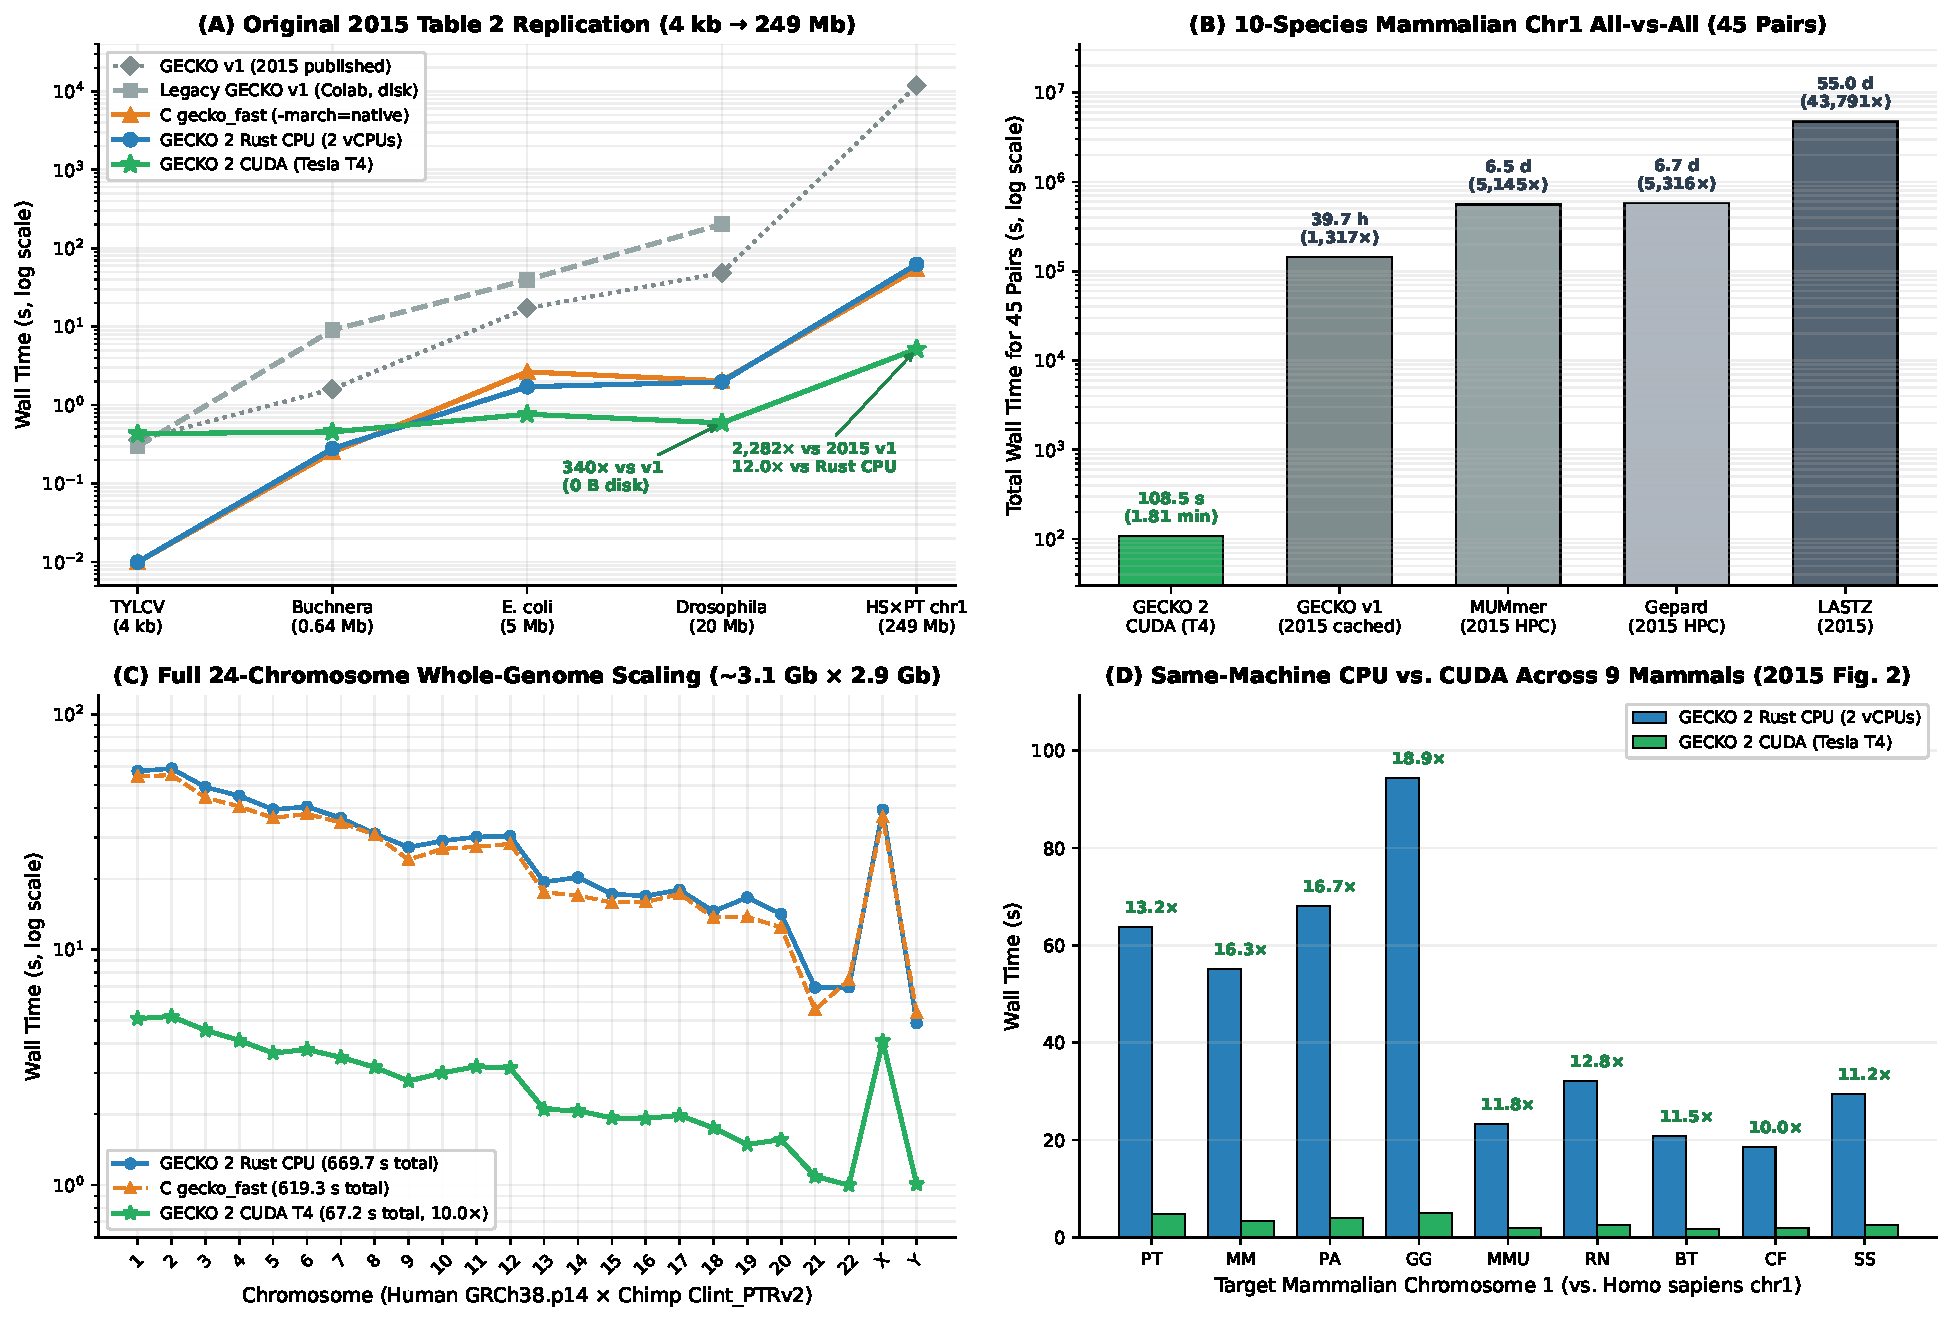
\includegraphics[width=\textwidth]{figures/gecko2_paper_figures.pdf}%
}{%
  \fbox{\parbox{0.96\textwidth}{\centering\vspace{1.8cm}\sffamily\footnotesize\color{orange!75!black}%
  \textbf{[Placeholder for Figure~2: \texttt{figures/gecko2\_paper\_figures.pdf}]}\\[4pt]
  Four-panel 300-DPI benchmark summary exported automatically by Cell~9 of the Colab notebook:\\
  (A)~Exp.~1 log-scale runtime (4~kb--249~Mb);\quad (B)~Exp.~2 45-pair mammalian all-vs-all vs.\ 2015 Table~4;\\
  (C)~Exp.~3 24-chr Human$\times$Chimp scaling;\quad (D)~Exp.~4A zero-spill slab memory scaling (\texttt{-m 512M..4G}).%
  \vspace{1.8cm}}}%
}
\caption{Comprehensive performance and memory scaling of GECKO~2 across all four experimental suites. \textbf{(A)} Direct replication of Torreno \& Trelles (2015) Table~2 across five orders of magnitude in sequence length (4~kb--249~Mb). \textbf{(B)} Aggregate runtime for all 45 pairwise comparisons of 10 mammalian chromosome~1 sequences compared against published 2015 benchmarks. \textbf{(C)} Per-chromosome scaling across all 24 human-versus-chimpanzee chromosome pairs. \textbf{(D)} Peak host RSS and wall-clock time on \textit{H.~sapiens} chr1 $\times$ \textit{P.~troglodytes} chr1 under strict \texttt{-m} memory budgets (0~MiB disk spillover).}\label{fig:results}
\end{figure}

%% ============================================================================
%% 4. DISCUSSION
%% ============================================================================
\section{Discussion}\label{sec:discussion}

\paragraph{Decomposing algorithmic versus hardware speedups.}
Including the intermediate \texttt{c\_fast} in-memory C baseline alongside \texttt{legacy\_v1}, Rust \texttt{cpu}, \texttt{wgpu}, and \texttt{cuda} cleanly separates two orthogonal sources of acceleration. First, replacing external disk sorting and dual-dictionary joins with single-reference canonical Hash-CSR streaming and 2-bit packed sequences delivers the largest single leap (over an order of magnitude on mammalian chromosomes) while dropping temporary disk I/O to zero. Second, Rust systems co-design --- 2-level 256-partition parallel radix indexing, non-polluting \texttt{\_MM\_HINT\_T2} prefetching, 2-tier diagonal caching, exact rejected-span skipping, and 2-bit SWAR/AVX2 extension --- outperforms \texttt{-O3 -march=native} C in a portable binary. Third, offloading indexing, maximal seed filtering, and two-tier warp-cooperative 2-bit extension to a commodity T4 GPU adds a further multi-fold acceleration, turning multi-day all-versus-all comparisons into single-digit-minute interactive runs.

\paragraph{CPU versus GPU crossover and backend trade-offs.}
On sub-megabase viral and small bacterial genomes (TYLCV, \textit{Buchnera}), GPU device initialization and PCIe transfers outweigh kernel compute time, making the Rust \texttt{cpu} backend the optimal choice (completing in milliseconds). Once sequences reach tens of megabases (\textit{Drosophila}, mammalian chromosomes) or hit density rises under short seeds ($\text{WL}=12$), GPU throughput dominates. Between the two GPU backends, native \texttt{cuda} consistently outperforms \texttt{wgpu} on NVIDIA hardware because CUDA natively supports 64-bit integer arithmetic, warp-level shuffle intrinsics (\texttt{\_\_shfl\_up\_sync}), and CUB device-wide radix sort, whereas \texttt{wgpu} must emulate 64-bit \texttt{fmix64} hashing via \texttt{vec2<u32>} and synchronize via Vulkan/WGSL compute barriers. Nevertheless, \texttt{wgpu} plays an essential role by delivering hardware GPU acceleration on Apple Silicon (Metal), AMD, and Intel GPUs where CUDA is unavailable.

\paragraph{Rethinking disk dictionary caching in all-versus-all studies.}
In 2015, a central rationale for GECKO~v1's disk-based design was reusing on-disk word dictionaries across $n(n-1)/2$ all-versus-all comparisons \cite{torreno2015gecko}. Experiment~2 reveals an important shift in modern hardware economics: rebuilding a 2-bit canonical index in GPU/host RAM on the fly for each pair is now orders of magnitude faster than deserializing gigabyte-scale hash tables from secondary storage. Even so, GECKO~2 retains optional \texttt{.gidx} caching via \texttt{gecko all-vs-all} and \texttt{--cache-dir}; keeping a reference slab index resident in GPU VRAM across all $n-1$ queries sharing the same reference is a straightforward future optimization that will compress all-versus-all runtimes even further.

\paragraph{Complementarity with sequence-to-function AI models and variant atlases.}
Recent deep learning sequence-to-function frameworks such as AlphaGenome \cite{avsec2026alphagenome} and its genome-wide human in silico mutagenesis catalog AlphaGenome Atlas \cite{cheng2026alphagenomeatlas} predict molecular and regulatory consequences (gene expression, splicing, chromatin state, and 3D contacts) across 1~Mb windows for every possible single-nucleotide substitution on the human reference genome. Such resources are fundamentally orthogonal and complementary to GECKO~2. Whereas sequence-to-function models rely on extensive species-specific epigenomic training tracks (primarily human and mouse) and evaluate local point variations on a fixed reference, GECKO~2 is entirely species-agnostic, requires zero training data, and deterministically discovers whole-chromosome structural rearrangements (inversions, duplications, translocations) and cross-species synteny blocks across arbitrary assemblies from viruses to 300~Mb chromosomes. In practice, the two paradigms reinforce one another: GECKO~2 can rapidly map conserved non-coding HSPs across mammalian genomes to prioritize evolutionary constraint alongside AlphaGenome Atlas impact scores, or pinpoint exact structural rearrangement breakpoints between primate and personal \textit{de novo} assemblies to identify the 1~Mb regulatory loci where sequence-to-function inference is most informative.

\paragraph{Limitations and future work.}
Because GECKO~2 currently performs FASTA/gzip parsing on the host CPU before device upload, disk read and parsing overhead accounts for a growing fraction of wall-clock time on fast GPUs (as visible in the gap between wall and compute times in Experiment~3). Future releases will address this I/O floor through parallel \texttt{bgzip} decoding and asynchronous double-buffered host-to-device slab streaming, alongside multi-GPU slab distribution for gigabase-scale plant chromosomes ($>$500~Mb per chromosome) and AVX-512 / ARM NEON intrinsics for 2-bit CPU extension.

%% ============================================================================
%% 5. CONCLUSIONS
%% ============================================================================
\section{Conclusions}\label{sec:conclusions}

GECKO~2 modernizes exhaustive ungapped whole-genome pairwise comparison by replacing out-of-core disk sorting with a zero-disk, memory-bounded, 2-bit streaming architecture in Rust with native CUDA and cross-vendor WebGPU acceleration. Directly replicating the original 2015 \textit{BMC Bioinformatics} benchmarks across viral, bacterial, insect, and mammalian genomes, GECKO~2 achieves \hlChrOneSpeedupCpuVsVone{} CPU and \hlChrOneSpeedupCudaVsVone{} GPU speedups on human--chimpanzee chromosome~1 while eliminating \hlChrOneVoneDiskGiB{} of temporary disk writes, completes the entire 45-pair 10-species mammalian chromosome~1 all-versus-all matrix in \hlAllVsAllCudaMin{} (down from 39.7~h in 2015), and compares all 24 human versus chimpanzee chromosomes in \hlWholeGenomeCudaSec{} on a commodity T4 GPU --- all with strict RAM bounds down to 512~MiB and drop-in legacy \texttt{.frags} compatibility.

%% ============================================================================
%% BMC BIOINFORMATICS MANDATORY BACKMATTER SECTIONS
%% ============================================================================
\backmatter

\section*{Availability and requirements}
\begin{itemize}
    \item \textbf{Project name:} GECKO~2
    \item \textbf{Project home page:} \url{https://github.com/otorreno/gecko}
    \item \textbf{Operating system(s):} Linux, macOS, Windows
    \item \textbf{Programming language:} Rust, CUDA C++, WGSL
    \item \textbf{Other requirements:} Rust toolchain ($\ge$1.85); optional NVIDIA CUDA Toolkit ($\ge$12.0) for \texttt{--features cuda}; Vulkan/Metal/DX12 driver for \texttt{--backend wgpu}
    \item \textbf{License:} GNU General Public License v3.0 (GPL-3.0)
    \item \textbf{Any restrictions to use by non-academics:} None beyond GPL-3.0
\end{itemize}

\section*{List of abbreviations}
CSR: Compressed Sparse Row; FL: Frequency Limit; GPU: Graphics Processing Unit; HSP: High-scoring Segment Pair; LCR: Low-Complexity Region; PAF: Pairwise mApping Format; RSS: Resident Set Size; SIMD: Single Instruction, Multiple Data; SWAR: SIMD Within A Register; WGSL: WebGPU Shading Language; WL: Word Length.

\section*{Declarations}

\subsection*{Ethics approval and consent to participate}
Not applicable.

\subsection*{Consent for publication}
Not applicable.

\subsection*{Availability of data and materials}
All genome sequences analyzed in this study are publicly available from NCBI GenBank/RefSeq under the exact accession numbers listed in Table~\ref{tab:datasets} and RefSeq assemblies \texttt{GCF\_000001405.40} (\textit{H.~sapiens} GRCh38.p14) and \texttt{GCF\_002880755.1} (\textit{P.~troglodytes} Clint\_PTRv2). The complete reproducible benchmark notebook is included in the project repository at \texttt{notebooks/gecko\_rust\_gpu\_benchmark.ipynb}.

\subsection*{Competing interests}
The authors declare that they have no competing interests.

\subsection*{Funding}
\tbd{Insert funding acknowledgments or ``Not applicable.''}

\subsection*{Authors' contributions}
O.Torreno designed and implemented the Rust, CUDA, and WebGPU architecture, designed and executed the benchmarks, and drafted the manuscript. O.Trelles supervised the study and contributed to methodological validation and manuscript revision. Both authors read and approved the final manuscript.

\subsection*{Acknowledgements}
\tbd{Insert acknowledgements or remove if not applicable.}

\bibliography{references}

\end{document}
